\documentclass{article}
\usepackage[utf8]{inputenc} %кодировка
\usepackage[T2A]{fontenc}
\usepackage[english,russian]{babel} %русификатор 
\usepackage{mathtools} %библиотека матеши
\usepackage[left=1cm,right=1cm,top=2cm,bottom=2cm,bindingoffset=0cm]{geometry} %изменение отступов на листе
\usepackage{amsmath}
\usepackage{graphicx} %библиотека для графики и картинок
\graphicspath{}
\DeclareGraphicsExtensions{.pdf,.png,.jpg}
\usepackage{subcaption}
\usepackage{pgfplots}
\usepackage{float}
\usepackage{hyperref}

\begin{document}
% НАЧАЛО ТИТУЛЬНОГО ЛИСТА
\begin{center}
    \Large
    Федеральное государственное автономное \\
    образовательное учреждение высшего образования \\ 
    «Научно-образовательная корпорация ИТМО»\\
    \vspace{0.5cm}
    \large
    Факультет программной инженерии и компьютерной техники \\
    Направление подготовки 09.03.04 Программная инженерия \\
    \vspace{1cm}
    \Large
    \textbf{Отчёт по лабораторной работе №2} \\
    По дисциплине «Информационные системы» ( семестр 5)\\
    \large
    \vspace{8cm}

    \begin{minipage}{.33\textwidth}
    \end{minipage}
    \hfill
    \begin{minipage}{.4\textwidth}
    
        \textbf{Студент}: \vspace{.1cm} \\
        \ Дениченко Александр P3312\\
        \textbf{Практик}:  \\
        \ Бострикова Д.К.
    \end{minipage}
    \vfill
Санкт-Петербург\\ 2024 г.
\end{center}
\pagestyle{empty}
% КОНЕЦ ТИТУЛЬНОГО ЛИСТА 
\newpage
\pagestyle{plain}

\section*{Задание}
\begin{center}
    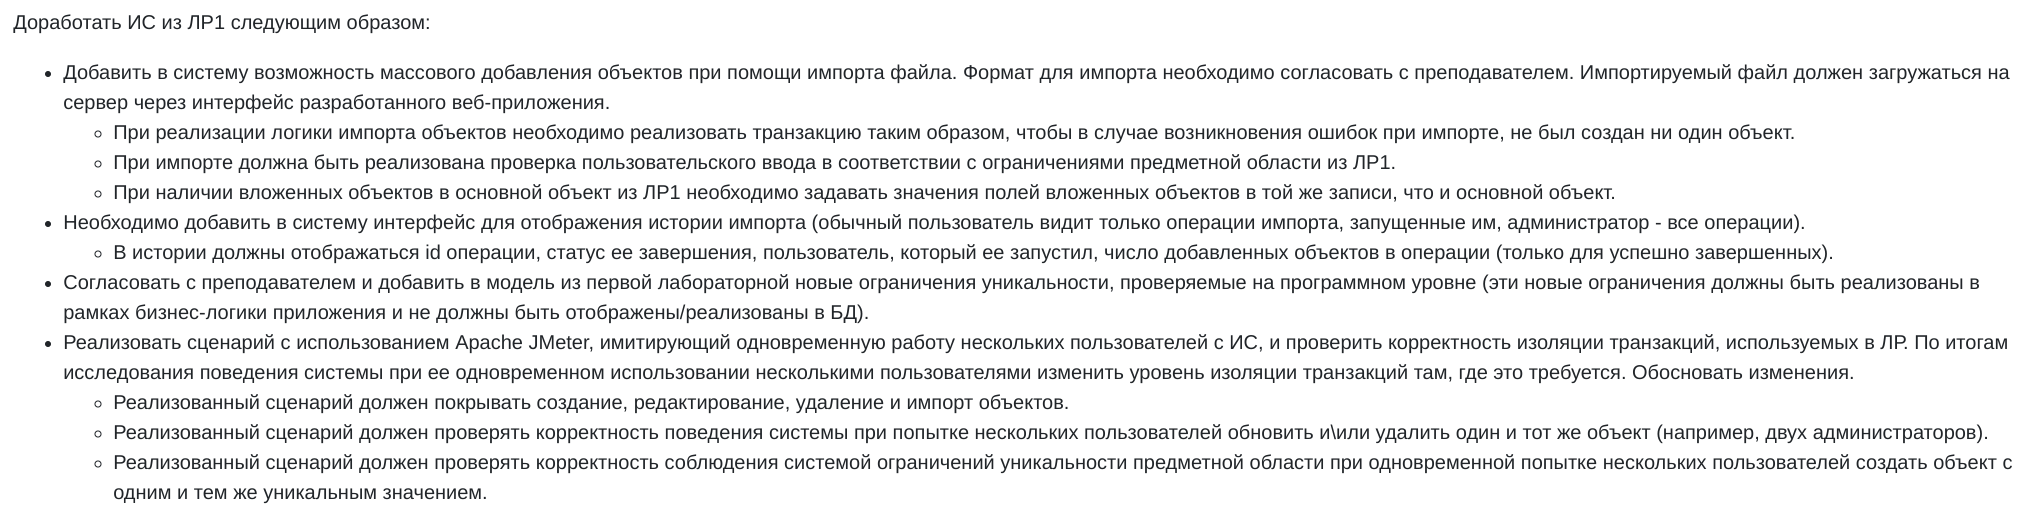
\includegraphics[width=.9\textwidth]{lab2}
\end{center}


\section{UML диаграммы}
    \subsection{Диаграмма пакетов}
        \begin{center}
            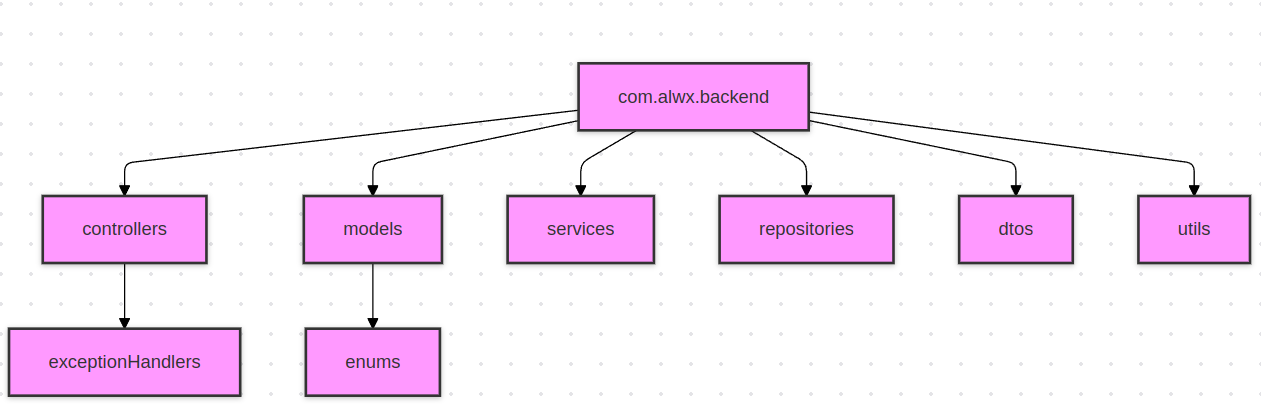
\includegraphics[width=.9\textwidth]{package_uml.png}
        \end{center}

\subsection{Диаграмма классов}
\href{https://www.mermaidchart.com/raw/7b97b9f2-bd1a-4381-be9d-0ba2c8f43344?theme=light&version=v0.1&format=svg}{Ссылка на диаграмму классов}

\section{Ссылка на проект}
\href{https://github.com/Alex-de-bug/Information-systems-itmo/tree/main/lab2spring}{Ссылка на проект}

\section{Выводы}
        В ходе выполнения лабораторной работы, были изучены основные принципы работы с транзакциями, их ошибками и исключениями.
        Так же был написан импорт файла с данными, который далее проходит в базу данных, так же действия касательно импортов логируются в базе данных.
\end{document}
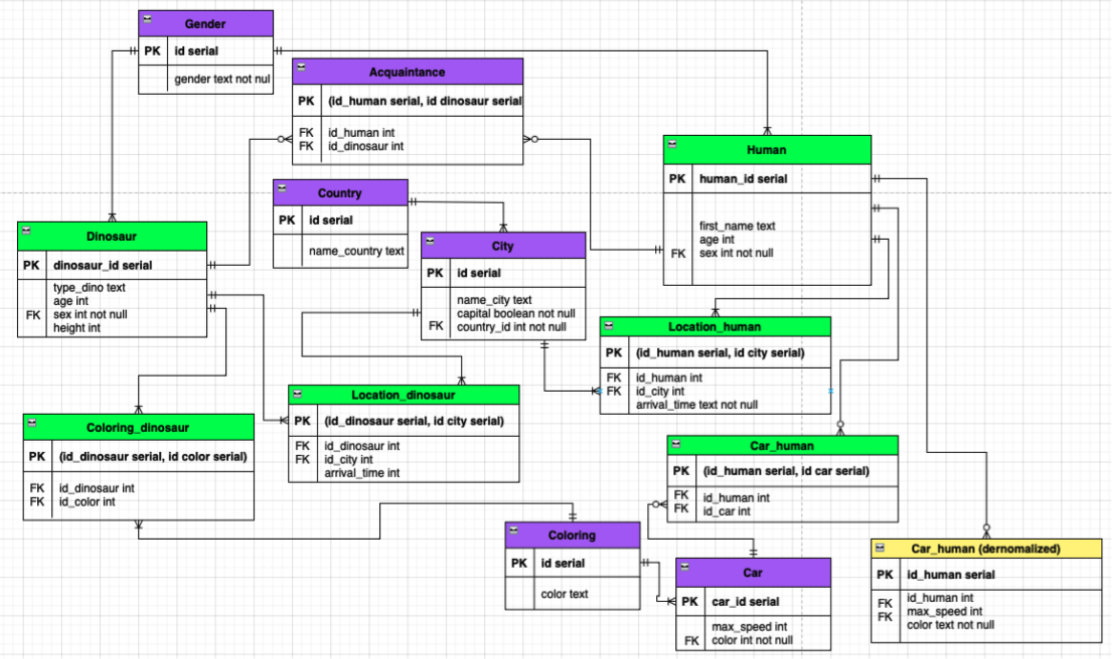
\includegraphics[width=.9\textwidth]{123}